% ============================================================
% QUDA MultiGrid 理解与 PyQCU 复现 — compact MATPC 增补汇报
% 编译：xelatex 两遍；交付闸门：Overfull=0, Float too large=0
% ============================================================
\documentclass[UTF8,aspectratio=169,11pt]{ctexbeamer}

\usepackage{amsmath,amssymb}
\usepackage{booktabs}
\usepackage{tabularx}
\usepackage{array}
\usepackage{tikz}
\usetikzlibrary{arrows.meta,positioning,calc,fit,shapes.geometric}
\usepackage{listings}
\usepackage{xcolor}
\usepackage{microtype}
\usepackage{hyperref}

\definecolor{primary}{HTML}{17365D}
\definecolor{accent}{HTML}{1F77B4}
\definecolor{evidence}{HTML}{1E8449}
\definecolor{warning}{HTML}{C55A11}
\definecolor{muted}{HTML}{5B6573}
\definecolor{panel}{HTML}{F4F7FA}
\definecolor{violet}{HTML}{6C4A9E}
\definecolor{good}{HTML}{EAF5EE}
\definecolor{warnbg}{HTML}{FFF4E8}

\setbeamersize{text margin left=0.55cm,text margin right=0.55cm}
\setlength{\columnsep}{0.30cm}
\setlength{\emergencystretch}{2em}
\setbeamertemplate{navigation symbols}{}
\setbeamertemplate{blocks}[rounded][shadow=false]
\setbeamercolor{normal text}{fg=black!86,bg=white}
\setbeamercolor{structure}{fg=primary}
\setbeamercolor{frametitle}{fg=primary,bg=white}
\setbeamercolor{block title}{fg=primary,bg=panel}
\setbeamercolor{block body}{fg=black!86,bg=panel}
\setbeamercolor{alerted text}{fg=warning}
\setbeamerfont{frametitle}{size=\large,series=\bfseries}
\setbeamerfont{normal text}{size=\normalsize}
\setbeamertemplate{frametitle}{\vskip0.12cm\insertframetitle\par\vskip0.08cm}
\setbeamertemplate{footline}{%
  \hbox{\begin{beamercolorbox}[wd=\paperwidth,ht=2.3ex,dp=0.9ex,
    leftskip=0.55cm,rightskip=0.55cm]{author in head/foot}%
    \scriptsize\color{muted}\insertshortauthor\hfill
    \insertshorttitle\hfill\insertframenumber/\inserttotalframenumber
  \end{beamercolorbox}}}

\newcolumntype{Y}{>{\raggedright\arraybackslash}X}
\newcolumntype{P}[1]{>{\raggedright\arraybackslash}p{#1}}
\newcommand{\source}[1]{%
  \vspace{0em}\par{\raggedright\fontsize{5.5pt}{6.5pt}\selectfont
  \color{muted}来源：#1\par}}
\newcommand{\codepath}[1]{%
  \ifmmode\text{\nolinkurl{#1}}%
  \else\nolinkurl{#1}\fi}
\newcommand{\verified}{\textcolor{evidence}{确证}}
\newcommand{\inferred}{\textcolor{accent}{推断}}
\newcommand{\unverified}{\textcolor{warning}{未验证}}

\tikzset{
  flow/.style={draw=accent,fill=accent!8,rounded corners=2pt,align=center,
    minimum height=0.58cm,text width=2.04cm,font=\small},
  state/.style={draw=primary,fill=primary!7,rounded corners=2pt,align=center,
    minimum height=0.58cm,text width=2.38cm,font=\small},
  phase/.style={draw=violet,fill=violet!8,rounded corners=2pt,align=center,
    minimum height=0.54cm,text width=2.03cm,font=\small},
  decision/.style={draw=warning,fill=warning!10,diamond,aspect=2.0,
    align=center,inner sep=1.2pt,font=\small},
  arrow/.style={-{Latex[length=2mm]},draw=primary,semithick},
  relation/.style={-{Latex[length=1.7mm]},draw=muted,thin,dashed},
  labelstyle/.style={font=\scriptsize,inner sep=1.5pt,fill=white,text=muted}
}

\lstset{
  basicstyle=\ttfamily\scriptsize,
  backgroundcolor=\color{panel},frame=single,
  breaklines=true,breakatwhitespace=false,keepspaces=true,
  columns=flexible,numbers=left,numberstyle=\tiny\color{muted},
  keywordstyle=\color{primary}\bfseries,
  commentstyle=\color{evidence!70!black},stringstyle=\color{accent}
}

\title[QUDA MG 复现]{QUDA MultiGrid 的算法理解与 PyQCU 复现}
\subtitle{MATPC 紧凑 odd Schur、P/R、Clover/Gauge 与旧实现对照}
\author[代码审计与代数验证]{代码审计与代数验证}
\institute{PyQCU · Lattice QCD}
\date{2026 年 8 月 29 日}

\begin{document}

\begin{frame}[plain]
  \titlepage
\end{frame}

\begin{frame}[t]{本轮结论：MATPC compact odd Schur 已进入新参考路径}
  \small
  \begin{columns}[T,totalwidth=\textwidth]
    \begin{column}{0.30\textwidth}
      \begin{block}{已完成}
        新增 \codepath{CompactParityLayout}、\codepath{CompactParityOperator}；
        \codepath{setup_operator="schur"} 首层构造 odd Schur，后续层直接 Galerkin 粗化。
      \end{block}
    \end{column}
    \begin{column}{0.30\textwidth}
      \begin{block}{本轮证据}
        定向命令与 \codepath{examples/pyqcu} 均为
        \textbf{26 passed}；compact 多层 full residual
        $1.02\times10^{-7}$，独立 Schur 解为 $1.12\times10^{-7}$。
      \end{block}
    \end{column}
    \begin{column}{0.30\textwidth}
      \begin{alertblock}{边界}
        旧 \codepath{solver.multigrid} 保留；当前交付是可验证的
        Python/CUDA 资产参考路径，不宣称 QUDA 生产 kernel 性能等价。
      \end{alertblock}
    \end{column}
  \end{columns}
  \vspace{0.25em}
  \begin{center}
    \begin{tikzpicture}[node distance=0.17cm and 0.17cm]
      \node[flow] (d) {完整 $D_f$};
      \node[flow,right=of d] (s) {一次\\$S_o$};
      \node[flow,right=of s] (p) {$P_0,R_0$};
      \node[flow,right=of p] (g) {$R_0S_oP_0$};
      \node[flow,right=of g] (r) {递归\\V-cycle};
      \draw[arrow] (d)--(s)--(p)--(g)--(r);
    \end{tikzpicture}
  \end{center}
  \vspace{0.18em}
  \colorbox{good}{\parbox{0.91\textwidth}{\textbf{阶段判断：}
    QUDA MATPC 的核心约束已落成可测不变量：奇偶布局、局部块逆、
    $S_o$ 严格伴随、$R S_o P$ 层级和 full 解重构均有回归证据。}}
  \source{实现：\codepath{pyqcu/solver/_quda_multigrid.py:1094-1292,1373-2331}；
    测试：\codepath{examples/pyqcu/test_quda_multigrid.py:434-725}；
    命令：\codepath{pytest -q examples/pyqcu}。}
\end{frame}

\begin{frame}[t]{研究问题与验收标准：先对齐代数，再谈加速}
  \footnotesize
  \begin{center}
    \renewcommand{\arraystretch}{0.78}
    \begin{tabularx}{0.95\textwidth}{@{}P{0.25\textwidth}Y P{0.22\textwidth}@{}}
      \toprule
      问题 & 本轮可检验定义 & 状态 \\
      \midrule
      QUDA 的层级如何递归？ & 每层由 $B\to V\to(P,R)\to D_c=RDP$，
        运行期再接 smoother、restrict、coarse solve、prolong。 & \verified \\
      Clover/Gauge 是否被保留？ & local Clover 进入 $X$，Gauge/hopping 进入
        $Y^\pm$；不能只粗化 hopping。 & \verified \\
      parity 是否只在最细层？ & MATPC 首层形成 $S_o$，后续在 odd 几何上继续
        $R S_o P$，不能重复减半。 & \verified \\
      PyQCU 是否可复现？ & compact/full round-trip、Schur adjoint、重构、
        Galerkin、求解和 QCU 资产 shape 全部回归。 & \verified \\
      性能是否等价？ & 需要 CUDA/MPI setup、混合精度和大格 benchmark；
        本轮不以 Python 小格代数替代性能证据。 & \unverified \\
      \bottomrule
    \end{tabularx}
  \end{center}
  \vspace{0.08em}
  \begin{block}{判定口径}
    \scriptsize
    直接运行的命令或恒等式为“确证”；从源码控制流推出的对应关系为“推断”；
    尚未在 QUDA/QCU 生产路径运行的项目明确标为“未验证”。
  \end{block}
  \source{对照：\codepath{quda/lib/multigrid.cpp}、\codepath{transfer.cpp}、
    \codepath{coarse_op.cuh}、\codepath{dirac_coarse.cpp}；日志：\codepath{logs/v20260829.txt}。}
\end{frame}

\begin{frame}[t]{QUDA 的递归控制流：reset 建层，operator 做一次 V-cycle}
  \footnotesize
  \begin{columns}[T,totalwidth=\textwidth]
    \begin{column}{0.51\textwidth}
      \begin{tabular}{@{}l@{}}
        $\text{输入： }D_\ell,\;B_\ell,\;\text{geometry},\;\text{precision}$\\
        $\text{reset：创建/刷新 }B_\ell\text{ 与 Transfer}_\ell$\\
        $\quad B_{\ell+1,i}\leftarrow R_\ell B_{\ell,i}\quad
          (\text{若不在各层重新生成})$\\
        $\text{createCoarseDirac：构造 coarse operator}$\\
        $\quad\text{区分 residual / smoother}$\\
        $\text{createCoarseSolver：封装 solver + MG}$\\
        $\text{operator：prepare}\to\text{pre-smooth}\to Rr\to\text{recurse}$\\
        $\quad\to Pe_c\to\text{post-smooth}$\\
        $\text{输出：full 或 MATPC solution，并按需要 reconstruct}$
      \end{tabular}
    \end{column}
    \begin{column}{0.39\textwidth}
      \begin{tikzpicture}[node distance=0.10cm]
        \node[state,font=\scriptsize,text width=2.55cm] (a) {细格 Dirac 与 B};
        \node[state,font=\scriptsize,text width=2.55cm,below=of a] (b) {Transfer / $RDP$};
        \node[state,font=\scriptsize,text width=2.55cm,below=of b] (c) {$X,Y$ 与 solver wrapper};
        \node[state,font=\scriptsize,text width=2.55cm,below=of c] (d) {递归 coarse MG};
        \draw[arrow] (a)--(b)--(c)--(d);
        \draw[relation] (d.east) -- ++(0.45,0) |- node[right=1pt,labelstyle]{返回校正}
          (b.east);
      \end{tikzpicture}
      \vspace{0.25em}
      \begin{block}{关键分离}
        \scriptsize
        QUDA 同时维护 residual operator、smoother operator 及 sloppy precision；
        它们必须在 solution type 不一致时显式重构并重算 residual。
      \end{block}
    \end{column}
  \end{columns}
  \source{QUDA：\codepath{multigrid.cpp:72-197}；
    PyQCU：\codepath{_quda_multigrid.py:1915-1986}。}
\end{frame}

\begin{frame}[t]{P/R 的本质：aggregate 几何 map 加 fine-spin 到 coarse-spin map}
  \footnotesize
  \begin{columns}[T,totalwidth=\textwidth]
    \begin{column}{0.45\textwidth}
      \begin{block}{几何与自由度}
        \begin{align*}
          a(x)&=\left(\left\lfloor x_0/b_0\right\rfloor,\ldots,
          \left\lfloor x_3/b_3\right\rfloor\right),\\
          q(s)&=\left\lfloor s/b_s\right\rfloor
          \quad\text{(Wilson/Clover)},\\
          D_f&=4\times3=12,\qquad D_c=2N_{\rm vec}.
        \end{align*}
        对 staggered，$b_s=0$，coarse spin 由 site parity 承载。
      \end{block}
    \end{column}
    \begin{column}{0.45\textwidth}
      \begin{block}{延拓与限制}
        \begin{align*}
          (P\eta)_{sc}(x)&=\sum_j V_{scqj}(x)\eta_{qj}(a(x)),\\
          (R\psi)_{qj}(a)&=\sum_{x\in a,s,c}
             V^*_{scqj}(x)\psi_{sc}(x),\\
          R&=P^\dagger,\qquad RP\simeq I_c.
        \end{align*}
        $V$ 只在同一 aggregate、同一 coarse-spin block 内正交。
      \end{block}
    \end{column}
  \end{columns}
  \vspace{-0.05em}
  \begin{center}
    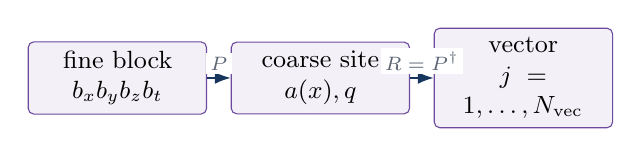
\begin{tikzpicture}[node distance=0.20cm and 0.30cm]
      \node[phase] (f) {fine block\\$b_xb_yb_zb_t$};
      \node[phase,right=of f] (m) {coarse site\\$a(x),q$};
      \node[phase,right=of m] (v) {vector\\$j=1,\ldots,N_{\rm vec}$};
      \draw[arrow] (f)--node[above=1pt,labelstyle]{$P$}(m);
      \draw[arrow] (m)--node[above=1pt,labelstyle]{$R=P^\dagger$}(v);
    \end{tikzpicture}
  \end{center}
  \vspace{-0.18em}
  \begin{center}
    \scriptsize\color{warning}\textbf{极限检查：}
    若 $N_{\rm vec}$ 超过 aggregate 局部维数，局部 CGS 无法产生独立列；
    容量约束是构建前硬条件。
  \end{center}
  \source{QUDA：\codepath{transfer.cpp:200-328}；
    PyQCU：\codepath{QudaTransfer}。}
\end{frame}

\begin{frame}[t]{块 CGS：局部正交化决定 $R=P^\dagger$ 是否数值可靠}
  \footnotesize
  \begin{columns}[T,totalwidth=\textwidth]
    \begin{column}{0.56\textwidth}
      \begin{tabular}{@{}l@{}}
        $\text{for each aggregate }a\text{ and coarse spin }q:$\\
        \quad $v_j\leftarrow B_j\quad(\text{first pass}),\qquad
          v_j\leftarrow V_j\quad(\text{later pass})$\\
        \quad $h_{ij}=\langle v_i,v_j\rangle_{a,q}$\\
        \quad $v_j\leftarrow v_j-\sum_{i<j}h_{ij}v_i$\\
        \quad $v_j\leftarrow v_j/\|v_j\|_{a,q}$\\
        $\text{repeat }n_{\rm block\_ortho}\text{ passes and save }V$
      \end{tabular}
      \vspace{0.25em}
      \begin{block}{局部维数}
        Wilson/Clover：$N_{\rm vec}\le N_c\,|a|\,b_s$；
        staggered：每个 coarse parity 只拥有 $N_c|a|/2$ 个位置。
      \end{block}
    \end{column}
    \begin{column}{0.34\textwidth}
      \begin{block}{PyQCU}
        \scriptsize
        \codepath{_cg_orthogonalise()} 按 block 批量执行重复 CGS；
        \codepath{QudaTransfer} 以相同的 $V$ 定义 prolong/restrict。
      \end{block}
      \begin{block}{当前直测}
        \scriptsize
        compact 两层例的最大 block Gram 误差：
        $4.34\times10^{-7}$；$RP$ 相对误差：
        $1.67\times10^{-7}$。
      \end{block}
    \end{column}
  \end{columns}
  \source{QUDA：\codepath{block_orthogonalize.cuh:149-239}；
    PyQCU：\codepath{_quda_multigrid.py:189-219,319-355}；
    直测：\codepath{QudaMultigrid.diagnostics()}。}
\end{frame}

\begin{frame}[t]{粗算子不是“只剩 dslash”：local Clover 与 Gauge hopping 都在 $RDP$}
  \footnotesize
  \begin{columns}[T,totalwidth=\textwidth]
    \begin{column}{0.44\textwidth}
      \begin{block}{Galerkin 定义}
        \begin{align*}
          D_{\ell+1}&=R_\ell D_\ell P_\ell,\\
          (D_cx)(q)&=X(q)x(q)\\
          &\quad+\sum_{\mu=0}^{3}\left[Y^+_\mu(q)x(q+\hat\mu)\right.\\
          &\qquad\left.+Y^-_\mu(q)x(q-\hat\mu)\right].
        \end{align*}
        $X$ 是目标点 local block；$Y^\pm$ 是带方向和边界约定的 hopping block。
      \end{block}
    \end{column}
    \begin{column}{0.46\textwidth}
      \begin{tabularx}{0.96\linewidth}{@{}P{0.24\linewidth}Y@{}}
        \toprule
        对象 & 实现语义 \\
        \midrule
        细层 Gauge & $U_\mu$ 进入 Wilson hopping；细层 $D_f$ 由 dslash 提供。\\
        细层 Clover & $C$ 进入 local $M$，参与 diagonal inverse。\\
        QUDA $Y$ & UV/VUV 累加 forward/backward link；必要时保留 halo。\\
        QUDA $X$ & coarse local Clover/identity；coarse-on-coarse 继续投影。\\
        PyQCU & materialize 逐列探测 $RDP$；lazy 执行 $R(D(Px))$。\\
        \bottomrule
      \end{tabularx}
    \end{column}
  \end{columns}
  \vspace{0.15em}
  \begin{alertblock}{物理一致性}
    丢掉 $X$ 会改变 Schur 补，丢掉 $Y$ 会改变传播；二者共同组成粗 Dirac
    operator，不能把粗层误写成不完备的 hopping-only dslash。
  \end{alertblock}
  \source{QUDA：\codepath{coarse_op.cuh}；
    PyQCU：\codepath{_quda_multigrid.py:664-910}。}
\end{frame}

\begin{frame}[t]{预条件粗算子：先构造 $X^{-1}$，再形成 $Yhat$ 与 Schur}
  \small
  \begin{columns}[T,totalwidth=\textwidth]
    \begin{column}{0.45\textwidth}
      \begin{block}{局部预条件}
        \begin{align*}
          D_c&=X+H,\qquad
          D_{\rm pc}=X^{-1}(D_c-X)\\
          &\quad=X^{-1}H,\\
          D_{\rm full,pc}&=X^{-1}D_c=I+D_{\rm pc},\\
          Yhat^+_\mu(q)&=X^{-1}(q)Y^+_\mu(q).
        \end{align*}
        backward link 存在存储位置平移，并带有伴随和右侧
        $X^{-\dagger}$ 的约定。
      \end{block}
    \end{column}
    \begin{column}{0.45\textwidth}
      \begin{tabular}{@{}P{0.98\linewidth}@{}}
        \codepath{DiracCoarsePC::Dslash}: 只施加 $D_{\rm pc}$\\
        \codepath{DiracCoarsePC::M}: even/odd Schur action\\
        \codepath{prepare/reconstruct}: full 与 MATPC solution 转换\\
        solution type 不一致：先 reconstruct，再重算 residual\\
        PyQCU: \codepath{preconditioned_apply} $\to$\\
        \quad\codepath{preconditioned_full_apply}
      \end{tabular}
      \vspace{0.25em}
      \begin{block}{实现检查}
        \scriptsize
        backward $Yhat$ 的索引、滚动方向和 $X^{-\dagger}$ 右因子必须同时正确；
        只验证 forward link 不足以证明 PC 算子正确。
      \end{block}
    \end{column}
  \end{columns}
  \source{QUDA：\codepath{coarse_op_preconditioned.cuh}；
    PyQCU：\codepath{_quda_multigrid.py:912-1056}。}
\end{frame}

\begin{frame}[t]{奇偶块代数：MATPC 的目标是 odd Schur，不是半截 full field}
  \small
  \begin{columns}[T,totalwidth=\textwidth]
    \begin{column}{0.47\textwidth}
      \begin{block}{块矩阵推导}
        \begin{equation*}
          D=\begin{pmatrix}D_{ee}&D_{eo}\\D_{oe}&D_{oo}\end{pmatrix},
          \qquad
          S_o=D_{oo}-D_{oe}D_{ee}^{-1}D_{eo}.
        \end{equation*}
        \begin{align*}
          b_o^S&=b_o-D_{oe}D_{ee}^{-1}b_e,\\
          x_e&=D_{ee}^{-1}(b_e-D_{eo}x_o).
        \end{align*}
        local diagonal $D_{ee}$ 是 Clover/identity block，必须可逆。
      \end{block}
    \end{column}
    \begin{column}{0.41\textwidth}
      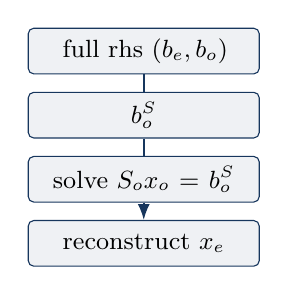
\begin{tikzpicture}[node distance=0.22cm]
        \node[state,text width=2.70cm] (b) {full rhs $(b_e,b_o)$};
        \node[state,text width=2.70cm,below=of b] (r) {$b_o^S$};
        \node[state,text width=2.70cm,below=of r] (s) {solve $S_ox_o=b_o^S$};
        \node[state,text width=2.70cm,below=of s] (x) {reconstruct $x_e$};
        \draw[arrow] (b)--(r)--(s)--(x);
      \end{tikzpicture}
      \vspace{0.22em}
      \begin{alertblock}{目标 parity}
        \scriptsize
        本轮固定保留 odd、消去 even；even-even 只需交换 parity 选择，
        公式结构不变。
      \end{alertblock}
    \end{column}
  \end{columns}
  \source{QUDA：\codepath{multigrid.cpp:1131-1224}、
    \codepath{dirac_coarse.cpp:506-626}；
    PyQCU：\codepath{_quda_multigrid.py:1295-1370}。}
\end{frame}

\begin{frame}[t]{compact parity 布局：$T$ 轴配对依赖空间 parity}
  \footnotesize
  \begin{columns}[T,totalwidth=\textwidth]
    \begin{column}{0.48\textwidth}
      \begin{block}{定义}
        完整场为 $[dof,X,Y,Z,T]$，紧凑 parity 场为
        $[dof,X,Y,Z,T/2]$。对空间 parity
        $e_s=(x+y+z)\bmod2$：
        \begin{align*}
          p&=(x+y+z+t)\bmod2,\\
          t_{\rm full}&=2t_{\rm half}
             +\bigl((p-x-y-z)\bmod2\bigr).
        \end{align*}
      \end{block}
      \begin{block}{两个具体分支}
        \begin{tabular}{@{}ll@{}}
          even $p=0$ & $t_{\rm full}=2t_{\rm half}+e_s$\\
          odd $p=1$ & $t_{\rm full}=2t_{\rm half}+(1-e_s)$
        \end{tabular}
      \end{block}
    \end{column}
    \begin{column}{0.40\textwidth}
      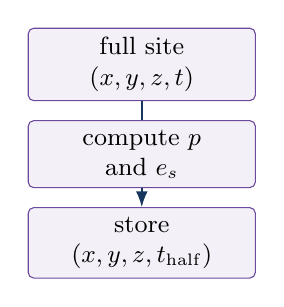
\begin{tikzpicture}[node distance=0.24cm]
        \node[phase,text width=2.65cm] (f) {full site\\$(x,y,z,t)$};
        \node[phase,text width=2.65cm,below=of f] (p) {compute $p$\\and $e_s$};
        \node[phase,text width=2.65cm,below=of p] (h) {store\\$(x,y,z,t_{\rm half})$};
        \draw[arrow] (f)--(p)--(h);
      \end{tikzpicture}
      \vspace{0.28em}
      \begin{alertblock}{硬约束}
        \scriptsize
        $T$ 必须为偶数；奇子格不是简单的“奇数 $t$”切片。
        该依赖若错一位，P/R 和每次 V-cycle 的残差都会失真。
      \end{alertblock}
    \end{column}
  \end{columns}
  \source{QCU 对照：\codepath{cpp/cuda/qcu/src/multigrid.cu:1579-1743}；
    PyQCU：\codepath{_quda_multigrid.py:1094-1161}；
    测试：\codepath{test_quda_multigrid.py:434-458}。}
\end{frame}

\begin{frame}[t]{新层级的关键决定：只做一次 finest Schur，粗层不再二次 checkerboard}
  \small
  \begin{center}
    \begin{tikzpicture}[node distance=0.26cm and 0.26cm]
      \node[flow,text width=2.30cm] (d) {完整 $D_f$\\$[12,X,Y,Z,T]$};
      \node[flow,text width=2.50cm,right=of d] (s) {一次 $S_o$\\$[12,X,Y,Z,T/2]$};
      \node[flow,text width=2.30cm,right=of s] (a) {$A_1=R_0S_oP_0$};
      \node[flow,text width=2.30cm,right=of a] (b) {$A_2=R_1A_1P_1$};
      \draw[arrow] (d)--(s)--(a)--(b);
    \end{tikzpicture}
  \end{center}
  \vspace{0.30em}
  \begin{columns}[T,totalwidth=\textwidth]
    \begin{column}{0.47\textwidth}
      \begin{block}{为什么不能再做 Schur}
        $S_o$ 已经只作用在 odd compact geometry。若对 $A_1$ 再调用旧
        checkerboard Schur，会把已有 $T/2$ 几何再次减半，得到错误的
        $T/4$ 层级；QUDA 的递归 MATPC 路径应直接 coarsen 当前算子。
      \end{block}
    \end{column}
    \begin{column}{0.41\textwidth}
      \begin{block}{自由度协议}
        full 模式的 \codepath{dof_list=[12,24,24]} 表示总 DOF，
        每个 coarse-spin block 用 $24/2=12$ 个向量；
        compact 模式条目直接作为当前 coarse DOF。
      \end{block}
    \end{column}
  \end{columns}
  \source{QUDA：\codepath{multigrid.cpp:347-434}；
    PyQCU：\codepath{_quda_multigrid.py:1691-1753}；compact 测试：\codepath{test_quda_multigrid.py}。}
\end{frame}

\begin{frame}[t]{compact Schur 的实现闭环：action、严格伴随、rhs 与 reconstruct}
  \footnotesize
  \begin{center}
    \begin{tabularx}{0.94\textwidth}{@{}P{0.23\textwidth}Y P{0.24\textwidth}@{}}
      \toprule
      接口 & 计算链 & 结果布局 \\
      \midrule
      \codepath{apply} &
        embed target odd $\to D_{oe}$；局部 $D_{ee}^{-1}$；
        再取 $D_{eo}$，最后减去 diagonal &
        $[dof,X,Y,Z,T/2]$ \\
      \codepath{adjoint_apply} &
        用完整 $D^\dagger$ 取相反块，并使用
        $(D_{ee}^{-1})^\dagger$；不假定 $S_o$ Hermitian &
        同上 \\
      \codepath{rhs} &
        $b_o-D_{oe}D_{ee}^{-1}b_e$ &
        odd compact rhs \\
      \codepath{reconstruct} &
        $x_e=D_{ee}^{-1}(b_e-D_{eo}x_o)$，再嵌回 full &
        $[dof,X,Y,Z,T]$ \\
      \bottomrule
    \end{tabularx}
  \end{center}
  \vspace{0.2em}
  \begin{block}{严格伴随的必要性}
    若 setup 选择 $D^\dagger D$，自定义 fine operator 必须提供
    \codepath{fine_adjoint}；Wilson/Clover 则自动使用
    $D^\dagger=\gamma_5D\gamma_5$。这是 setup 与 Schur adjoint 共用的同一物理对称性。
  \end{block}
  \source{PyQCU：\codepath{_quda_multigrid.py:579-661,1164-1292}；
    测试：\codepath{test_quda_multigrid.py:460-505}。}
\end{frame}

\begin{frame}[t]{setup 与求解：compact 只改变算子空间，不改变外层验证语义}
  \footnotesize
  \begin{columns}[T,totalwidth=\textwidth]
    \begin{column}{0.52\textwidth}
      \begin{tabular}{@{}P{0.98\linewidth}@{}}
        $\text{random：直接使用随机/显式 }B$\\
        $\text{inverse/null：求 }A\delta=AB,\quad B\leftarrow B-\delta$\\
        $\text{test：从零初值求 }A B_{\rm new}=B$\\
        $\text{cg/ca-cg：默认 }A=D^\dagger D$\\
        $\text{krylov/gcr：默认直接作用于非厄米 }D$\\
        compact 首层：$A=S_o$；\\
        \quad 后续层：$A=R S_o P$（当前 coarse op）
      \end{tabular}
    \end{column}
    \begin{column}{0.38\textwidth}
      \begin{block}{外层 solve}
        \scriptsize
        \begin{align*}
          b&\to b_o^S,\\
          x_o&\leftarrow\mathrm{FGMRES}
             (S_o,\;V\text{-cycle}),\\
          x&\to\mathrm{reconstruct}(b,x_o).
        \end{align*}
        公共 \codepath{apply} 仍返回 full $D$；另有
        \codepath{apply_compact} 返回 $S_o$。
      \end{block}
      \begin{alertblock}{验证}
        \scriptsize
        \codepath{TEST_VECTOR_SETUP} 对 $D=2I$ 得到精确的 $B/2$；
        compact setup history 显式记录首层 operator 为 Schur。
      \end{alertblock}
    \end{column}
  \end{columns}
  \source{PyQCU：\codepath{_quda_multigrid.py:1728-1903}；
    测试：\codepath{test_quda_multigrid.py:506-525}。}
\end{frame}

\begin{frame}[t]{V-cycle 的 compact 语义：coarse solve 直接作用在当前 Galerkin 算子}
  \small
  \begin{columns}[T,totalwidth=\textwidth]
    \begin{column}{0.52\textwidth}
      \begin{tabular}{@{}l@{}}
        $r_\ell=b_\ell-A_\ell x_\ell$\\
        $x_\ell\leftarrow\mathrm{MR}(A_\ell,r_\ell)$\\
        $r_{\ell+1}\leftarrow R_\ell r_\ell$\\
        $e_{\ell+1}\leftarrow\mathrm{solve}(A_{\ell+1},r_{\ell+1})$\\
        $x_\ell\leftarrow x_\ell+P_\ell e_{\ell+1}$\\
        $x_\ell\leftarrow\mathrm{MR}(A_\ell,r_\ell,x_\ell)$\\
        $K(r_\ell)=x_\ell\quad\text{作为 FGMRES 右预条件器}$
      \end{tabular}
    \end{column}
    \begin{column}{0.39\textwidth}
      \begin{tikzpicture}[node distance=0.10cm]
        \node[flow,text width=2.22cm,font=\scriptsize] (p) {pre-smooth};
        \node[flow,text width=2.22cm,font=\scriptsize,below=of p] (r) {$Rr$};
        \node[flow,text width=2.22cm,font=\scriptsize,below=of r] (c) {直接 coarse solve};
        \node[flow,text width=2.22cm,font=\scriptsize,below=of c] (q) {$Pe_c$};
        \node[flow,text width=2.22cm,font=\scriptsize,below=of q] (s) {post-smooth};
        \draw[arrow] (p)--(r)--(c)--(q)--(s);
      \end{tikzpicture}
      \vspace{0.22em}
      \begin{block}{防止重复减半}
        \scriptsize
        compact 分支的 smoother 与底层 solve 直接调用
        \codepath{operator.apply}；不再访问旧
        \codepath{ParitySchurOperator}。
      \end{block}
    \end{column}
  \end{columns}
  \source{PyQCU：\codepath{_quda_multigrid.py:2053-2133}；
    QUDA 运行期对照：\codepath{multigrid.cpp:1131-1224}。}
\end{frame}

\begin{frame}[t]{QCU 过渡资产：blocked P/R 与 33 点 stencil 都携带 compact 元数据}
  \scriptsize
  \begin{columns}[T,totalwidth=\textwidth]
    \begin{column}{0.48\textwidth}
      \begin{block}{P/R ABI}
        \begin{align*}
          V_{\rm Python}&:[s,c,q,j,X,Y,Z,T],\\
          V_{\rm QCU}&:[E,e,X_c,b_x,Y_c,b_y,Z_c,b_z,T_c,b_t],\\
          E&=N_{\rm coarse\ spin}N_{\rm vec},\quad
          e=N_{\rm fine\ spin}N_{\rm fine\ color}.
        \end{align*}
        \codepath{to_qcu_blocked()} 只做轴重排和 aggregate 拆分；
        $R$ 的共轭不被写入 $P$。
      \end{block}
      \begin{block}{资产元数据}
        \codepath{compact_parity}、\codepath{parity}、
        \codepath{eliminated_parity}、\codepath{fine_full_shape}、
        \codepath{fine/coarse_dof} 和 \codepath{operator_kind}。
      \end{block}
    \end{column}
    \begin{column}{0.43\textwidth}
      \begin{block}{33 点槽位}
        \begin{tabular}{@{}ll@{}}
          \codepath{sitting} & $(0,0,0,0)$\\
          \codepath{hop_nn} & $\pm\hat\mu,\;\mu=0,\ldots,3$\\
          \codepath{hop_diag} & $\pm\hat\mu\pm\hat\nu$，六个 pair
        \end{tabular}
        \vspace{0.12em}

        extent $=2$ 的重复邻居平均分到两个符号槽；
        extent $=1$ 折入 sitting；strict 模式拒绝更宽支撑。
      \end{block}
      \begin{alertblock}{本轮 compact 标识}
        \codepath{level=0}: \codepath{compact_schur}；
        后续 level: \codepath{compact_galerkin}。
        这明确禁止把 coarse transition 当成二次 Schur。
      \end{alertblock}
    \end{column}
  \end{columns}
  \source{PyQCU：\codepath{_quda_multigrid.py:446-470,817-910,2135-2191}；
    QCU 对照：\codepath{cpp/cuda/qcu/src/multigrid.cu:858-874}。}
\end{frame}

\begin{frame}[t]{旧实现与新实现并存：新路径补齐语义，不静默替换历史基线}
  \footnotesize
  \begin{center}
    \begin{tabularx}{0.96\textwidth}{@{}P{0.21\textwidth}YY@{}}
      \toprule
      维度 & 旧 \codepath{solver.multigrid} & 新 \codepath{solver.QudaMultigrid} \\
      \midrule
      MG-0 parity & 保留已有 fine/最细层 parity 行为 & 首层显式 compact odd $S_o$ \\
      粗层算子 & 历史路径的粗层未完整表达 full dslash，作为对照 & 每层 $D_{l+1}=R_lD_lP_l$，支持 lazy/materialize \\
      粗层 parity & 未延伸为完整递归 compact MATPC & 后续层直接在 compact 几何上 Galerkin，不二次减半 \\
      Clover/Gauge & 依赖旧接口与历史约定 & 细层复用 Wilson/Clover；local $X$ 和 hopping $Y$ 均保留 \\
      P/R & 历史扁平 $E$ 约定 & 显式 coarse spin、局部 CGS、$R=P^\dagger$ 和 QCU blocked 导出 \\
      角色 & 历史/生产实验基线，不能删除 & QUDA 语义参考与迁移验证基线 \\
      \bottomrule
    \end{tabularx}
  \end{center}
  \vspace{0.15em}
  \begin{block}{兼容策略}
    \scriptsize
    \codepath{pyqcu/solver/__init__.py} 同时导出旧类与
    \codepath{QudaMultigrid}、\codepath{CompactParityLayout}、
    \codepath{CompactParityOperator}；测试明确断言新旧导出不是同一类。
  \end{block}
  \source{旧实现：\codepath{pyqcu/solver/_multigrid.py}；
    新实现：\codepath{pyqcu/solver/_quda_multigrid.py}；
    导出：\codepath{pyqcu/solver/__init__.py:1-14}；
    测试：\codepath{test_quda_multigrid.py:101-104}。}
\end{frame}

\begin{frame}[t]{本轮代数证据：布局、Schur、Galerkin 与求解均通过}
  \scriptsize
  \begin{columns}[T,totalwidth=\textwidth]
    \begin{column}{0.49\textwidth}
      \begin{tabularx}{0.96\linewidth}{@{}Y r@{}}
        \toprule
        指标（$4^4$，complex64） & 实测 \\
        \midrule
        compact $RP$ 相对误差 & $1.67\times10^{-7}$ \\
        transfer 伴随相对误差 & $6.76\times10^{-9}$ \\
        compact block Gram 最大误差 & $4.34\times10^{-7}$ \\
        $R S_o P$ Galerkin 相对误差 & $7.81\times10^{-8}$ \\
        Schur 严格伴随内积误差 & $5.45\times10^{-9}$ \\
        eliminated-even 重构误差 & $2.18\times10^{-8}$ \\
        \bottomrule
      \end{tabularx}
    \end{column}
    \begin{column}{0.40\textwidth}
      \begin{tabularx}{0.96\linewidth}{@{}Y r@{}}
        \toprule
        compact 求解/资产 & 实测 \\
        \midrule
        MG full residual & $1.02\times10^{-7}$ \\
        direct Schur residual & $1.12\times10^{-7}$ \\
        $S_o$ 与 dslash parity action & $0$ \\
        operator DOF & $12,2,2$ \\
        asset kind & Schur / Galerkin \\
        目录级回归 & $26/26$ \\
        \bottomrule
      \end{tabularx}
      \vspace{0.15em}
      \begin{block}{解释}
        \scriptsize
        compact projection residual 不要求任意随机 full field 被 $P P^\dagger$
        精确表示；本轮验收的是 $RP$、adjoint、Galerkin 和 full residual。
      \end{block}
    \end{column}
  \end{columns}
  \vspace{0.12em}
  \begin{alertblock}{证据含义}
    这些数字证明 Python 参考实现的代数和布局约定；它们不等价于 GPU
    kernel 吞吐、MPI scaling 或 QUDA 原生数值路径的性能结论。
  \end{alertblock}
  \source{命令：定向测试与 \codepath{examples/pyqcu} 均 26 passed；
    数值：compact 直测。}
\end{frame}

\begin{frame}[t]{测试覆盖已扩展到物理输入：Wilson、Clover 与 Gauge 均进入 compact setup}
  \small
  \begin{columns}[T,totalwidth=\textwidth]
    \begin{column}{0.49\textwidth}
      \begin{block}{测试矩阵}
        \begin{tabularx}{0.96\linewidth}{@{}P{0.34\linewidth}Y@{}}
          输入 & 验证内容 \\
          \midrule
          identity diagonal & TEST setup 的 $S=2I$ 精确缩放 \\
          Wilson + $U=I$ & parity action = compact Schur \\
          Wilson + random Gauge & setup / $RDP$ / reconstruct \\
          Wilson + Clover $C$ & local inverse / Schur reconstruct \\
          两层 compact hierarchy & solve / QCU asset shape \\
        \end{tabularx}
      \end{block}
    \end{column}
    \begin{column}{0.41\textwidth}
      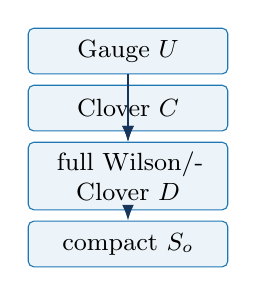
\begin{tikzpicture}[node distance=0.13cm]
        \node[flow,text width=2.30cm] (u) {Gauge $U$};
        \node[flow,text width=2.30cm,below=of u] (c) {Clover $C$};
        \node[flow,text width=2.30cm,below=of c] (d) {full Wilson/Clover $D$};
        \node[flow,text width=2.30cm,below=of d] (s) {compact $S_o$};
        \draw[arrow] (u)--(d);
        \draw[arrow] (c)--(d);
        \draw[arrow] (d)--(s);
      \end{tikzpicture}
      \vspace{0.24em}
      \begin{alertblock}{直接结果}
        \scriptsize
        同一测试函数对 \codepath{clover_term=None} 与显式 local Clover
        均通过 \codepath{transfer_RP}、\codepath{galerkin_RDP} 和
        \codepath{schur_reconstruct_even}。
      \end{alertblock}
    \end{column}
  \end{columns}
  \source{测试：\codepath{test_quda_multigrid.py:694-725}；
    细层接口：\codepath{_quda_multigrid.py:1490-1531}。}
\end{frame}

\begin{frame}[t]{当前限制与风险：代数闭环不等于生产性能闭环}
  \footnotesize
  \begin{center}
    \begin{tabularx}{0.95\textwidth}{@{}P{0.30\textwidth}P{0.31\textwidth}Y@{}}
      \toprule
      项目 & 当前状态 & 影响与下一步 \\
      \midrule
      coarse materialize & 小格可逐列保存；大格有元素上限，推荐 lazy/批量 stencil &
        不能用逐列 Python 探测估计生产 setup 成本。 \\
      compact Schur & Python action、adjoint、setup、solve 已验证 &
        仍需接入 QCU production setup 并做 device/MPI full residual。 \\
      33 点支撑 & QCU stencil 有 strict guard &
        超出 nearest/diagonal 支撑时必须改 kernel 或保留 matrix-free，不能静默截断。 \\
      精度/通信 & 本轮为 CPU complex64 小格 &
        混合精度、ghost、MPI 拓扑和大格 scaling 未由本轮新测试覆盖。 \\
      性能结论 & 没有本轮 benchmark &
        不报告相对 QUDA 的吞吐、setup 时间或迭代数收益。 \\
      \bottomrule
    \end{tabularx}
  \end{center}
  \vspace{0.18em}
  \colorbox{warnbg}{\parbox{0.91\textwidth}{\textbf{风险控制：}
    所有未运行项目保持“未验证”标签；先以 compact layout、Schur、
    $RDP$ 和真残差作为迁移的 golden contract，再进入 CUDA/MPI 性能实验。}}
  \source{实现边界：\codepath{_quda_multigrid.py:748-910,2145-2163}；
    QCU 既有证据与历史结果见 \codepath{examples/qcu/dev87/}。}
\end{frame}

\begin{frame}[t]{阶段结论与后续：先完成 QCU compact 接线，再量化收益}
  \small
  \begin{columns}[T,totalwidth=\textwidth]
    \begin{column}{0.30\textwidth}
      \begin{block}{已确认}
        \begin{minipage}{0.95\linewidth}
          \scriptsize
          \begin{itemize}
            \item QUDA 层级主线为 $B\to V\to P/R\to RDP$；
            \item $X$、$Y$、$X^{-1}$、$Yhat$ 和 parity 是同一粗算子体系；
            \item compact MATPC 只在 finest 做一次 odd Schur。
          \end{itemize}
        \end{minipage}
      \end{block}
    \end{column}
    \begin{column}{0.30\textwidth}
      \begin{block}{本轮交付}
        \scriptsize
        新类、导出、26 项回归、compact QCU asset metadata，以及本报告
        \codepath{report_quda_multigrid_reproduction_20260829_4.tex/.pdf}。
      \end{block}
      \begin{alertblock}{旧路径}
        \scriptsize
        \codepath{pyqcu/solver/_multigrid.py} 保留为缺陷/历史对照，不做无声替换。
      \end{alertblock}
    \end{column}
    \begin{column}{0.30\textwidth}
      \begin{block}{下一阶段验收}
        \scriptsize
        \begin{tabular}{@{}P{0.98\linewidth}@{}}
          1. compact asset 接 QCU production setup；\\
          2. 2/4 rank full residual + parity round-trip；\\
          3. 大格 setup/solve 时间、迭代数与显存；\\
          4. QUDA 原生 kernel 同口径对照。
        \end{tabular}
      \end{block}
    \end{column}
  \end{columns}
  \vspace{0.30em}
  \begin{center}
    \begin{tikzpicture}[node distance=0.28cm and 0.28cm]
      \node[phase] (a) {代数 golden contract};
      \node[phase,right=of a] (b) {QCU compact setup};
      \node[phase,right=of b] (c) {MPI 真残差};
      \node[phase,right=of c] (d) {大格 benchmark};
      \draw[arrow] (a)--(b)--(c)--(d);
    \end{tikzpicture}
  \end{center}
  \source{行动依据：本轮 compact 代数测试与日志 \codepath{v20260829.txt}；
    性能/资源节点尚未排期。}
\end{frame}

\appendix

\begin{frame}[t]{附录：对象—源码—证据索引}
  \scriptsize
  \begin{center}
    \renewcommand{\arraystretch}{0.88}
    \begin{tabularx}{0.96\textwidth}{@{}P{0.23\textwidth}P{0.38\textwidth}Y@{}}
      \toprule
      对象 & QUDA 对照 & PyQCU 当前证据 \\
      \midrule
      递归 MG & \codepath{multigrid.cpp:72-197,1131-1224} &
        \codepath{QudaMultigrid.setup/v_cycle} \\
      geometry/spin map & \codepath{transfer.cpp:200-257} &
        \codepath{QudaTransfer}，含 Wilson/staggered \\
      P/R & \codepath{transfer.cpp:259-328} &
        局部 CGS、$R=P^\dagger$、QCU blocked export \\
      coarse $X/Y$ & \codepath{coarse_op.cuh:1035-1459} &
        materialized/lazy $RDP$、33 点打包 \\
      PC/Yhat & \codepath{dirac_coarse.cpp:351-430,506-626} &
        \codepath{preconditioned_apply} 与 local inverse \\
      parity & \codepath{multigrid.cpp:1131-1224} &
        \codepath{ParitySchurOperator} 与 compact Schur \\
      compact map & QCU \codepath{multigrid.cu:1579-1743} &
        \codepath{CompactParityLayout} 与 round-trip 测试 \\
      旧实现 & PyQCU 历史路径 & \codepath{solver/_multigrid.py} 未替换 \\
      \bottomrule
    \end{tabularx}
  \end{center}
  \vspace{0.25em}
  \begin{block}{证据等级}
    \verified：本轮命令或数值直测；\inferred：源码控制流和代数推导的一致性判断；
    \unverified：尚未运行的生产 setup、MPI、混合精度或性能项目。
  \end{block}
  \source{工作目录：\codepath{/root/PyQCU}；对照目录：
    \codepath{/root/PyQCU/refer/git-rep/quda}。}
\end{frame}

\begin{frame}[t,fragile]{附录：最小调用与 compact API}
  \footnotesize
  \begin{columns}[T,totalwidth=\textwidth]
    \begin{column}{0.55\textwidth}
      \begin{lstlisting}[language=Python,aboveskip=0.2em,belowskip=0.2em]
from pyqcu.solver import QudaMultigrid

mg = QudaMultigrid(
    U=U, clover_term=C, kappa=kappa,
    null_vectors=[B0, B1],
    block_size=[(2,2,2,2), (1,1,1,1)],
    max_level=3, use_parity=True,
    setup_operator="schur")
x = mg.solve(b)
Sbo = mg.apply_compact(bo)
assets = mg.qcu_transition_assets()
      \end{lstlisting}
    \end{column}
    \begin{column}{0.35\textwidth}
      \begin{block}{输入约定}
        \scriptsize
        \codepath{b}: full $[4,3,X,Y,Z,T]$ 或 flat $[12,X,Y,Z,T]$；
        \codepath{apply_compact}: odd $[12,X,Y,Z,T/2]$；
        \codepath{assets}: 每条 transition 的 blocked $P$ 与 stencil。
      \end{block}
      \begin{alertblock}{注意}
        \scriptsize
        $T$ 必须偶数；自定义 operator 启用 normal setup 时须显式提供
        \codepath{fine_adjoint} 和 parity 所需 \codepath{fine_diagonal}。
      \end{alertblock}
    \end{column}
  \end{columns}
  \source{接口：\codepath{pyqcu/solver/_quda_multigrid.py:1400-1544,2021-2034,2135-2191}。}
\end{frame}

\begin{frame}[t]{附录：本轮验证命令与交付闸门}
  \small
  \begin{tabular}{@{}l@{}}
    \texttt{\$ pytest -q examples/pyqcu/test\_quda\_multigrid.py}
      \quad\textbf{26 passed in 8.22s}\\
    \texttt{\$ pytest -q examples/pyqcu}
      \quad\textbf{26 passed in 8.99s}\\
    \texttt{\$ python -m py\_compile ...}
      \quad\textbf{通过}\\
    \texttt{\$ git diff --check}
      \quad\textbf{通过}\\
    \texttt{\$ xelatex ... (two passes)}
      \quad\textbf{Overfull=0, Float too large=0}\\
    \texttt{\$ pdfinfo / pdftoppm}
      \quad\textbf{页数一致，逐页渲染检查通过}
  \end{tabular}
  \vspace{0.35em}
  \begin{block}{交付判定}
    页面数、渲染页数和逐页检查数必须一致；报告中的“确证”只对应上表
    或前述可复查源码/恒等式证据。性能、生产 setup 和多 rank compact
    结果在本轮保持未验证。
  \end{block}
  \source{文件：\codepath{docs/report_quda_multigrid_reproduction_20260829_4.tex/.pdf}；
    Git 收尾将在报告编译与渲染检查后执行。}
\end{frame}

\end{document}
